\def\duedate{\today}
\def\HWnum{9}
\documentclass[10pt,a4paper]{book}

% custom section formatting
\usepackage{titlesec}
\titleformat{\chapter}[display]
{\normalfont\Large\filcenter\sffamily}
{\titlerule[1pt]%
\vspace{1pt}%
\titlerule
\vspace{1pc}%
\LARGE\MakeUppercase{\chaptertitlename} \thechapter}
{1pc}
{\titlerule
\vspace{1pc}%
\Huge}

% appendix handling
\usepackage[toc,page]{appendix}
    
% encoding for file and font
\usepackage[utf8]{inputenc}
\usepackage[T1]{fontenc}

% math formatting/tools
\usepackage{amsmath}
\usepackage{amssymb}
\usepackage{mathtools}
\usepackage[arrowdel]{physics}

% unit formatting
\usepackage{siunitx}
\AtBeginDocument{\RenewCommandCopy\qty\SI}

% figure formatting/tools
\usepackage{graphicx}
\usepackage{float}
\usepackage{subcaption}
\usepackage{multirow}
\usepackage{import}
\usepackage{pdfpages}
\usepackage{transparent}
\usepackage{currfile}

\NewDocumentCommand\incfig{O{1} m}{
    \def\svgwidth{#1\textwidth}
    \import{./Figures/\currfiledir}{#2.pdf_tex}
}

\newcommand{\bef}{\begin{figure}[h!tb]\centering}
\newcommand{\eef}{\end{figure}}

\newcommand{\bet}{\begin{table}[h!tb]\centering}
\newcommand{\eet}{\end{table}}

% hyperlink references 
\usepackage{hyperref}
\hypersetup{
    colorlinks=true,
    linkcolor=blue,
    filecolor=magenta,
    urlcolor=cyan,
    pdftitle={Physics 1 Notes},
    pdfauthor={Richard Whitehill},
    pdfpagemode=FullScreen
}
\urlstyle{same}

\newcommand{\eref}[1]{Eq.~(\ref{eq:#1})}
\newcommand{\erefs}[2]{Eqs.~(\ref{eq:#1})--(\ref{eq:#2})}

\newcommand{\fref}[1]{Fig.~(\ref{fig:#1})}
\newcommand{\frefs}[2]{Fig.~(\ref{fig:#1})--(\ref{fig:#2})}

\newcommand{\aref}[1]{Appendix~(\ref{app:#1})}
\newcommand{\sref}[1]{Section~(\ref{sec:#1})}
\newcommand{\srefs}[2]{Sections~(\ref{sec:#1})-(\ref{sec:#2})}

\newcommand{\tref}[1]{Table~(\ref{tab:#1})}
\newcommand{\trefs}[2]{Table~(\ref{tab:#1})--(\ref{tab:#2})}

% tcolorbox formatting/definitions
\usepackage[most]{tcolorbox}
\usepackage{xcolor}
\usepackage{xifthen}
\usepackage{parskip}

\definecolor{peach}{rgb}{1.0,0.8,0.64}

\DeclareTColorBox[auto counter, number within=chapter]{defbox}{O{}}{
    enhanced,
    boxrule=0pt,
    frame hidden,
    borderline west={4pt}{0pt}{green!50!black},
    colback=green!5,
    before upper=\textbf{Definition \thetcbcounter \ifthenelse{\isempty{#1}}{}{: #1} \\ },
    sharp corners
}

\newcommand*{\eqbox}{\tcboxmath[
    enhanced,
    colback=black!10!white,
    colframe=black,
    sharp corners,
    size=fbox,
    boxsep=8pt,
    boxrule=1pt
]}

\newtcolorbox[auto counter, number within=chapter]{exbox}{
    parbox=false,
    breakable,
    enhanced,
    sharp corners,
    boxrule=1pt,
    colback=white,
    colframe=black,
    before upper= \textbf{Example \thetcbcounter:}\,,
    before lower= \textbf{Solution:}\,,
    segmentation hidden
}

\newtcolorbox{resbox}{
    enhanced,
    colback=black!10!white,
    colframe=black,
    boxrule=1pt,
    boxsep=0pt,
    top=2pt,
    ams nodisplayskip,
    sharp corners
}


\begin{document}

\prob{1}{

A localized distribution of charge has a charge density
\begin{eqnarray}
    \rho(\va*{r}) = \frac{1}{64 \pi} r^2 e^{-r} \sin^2{\theta}
.\end{eqnarray}

(a) Make a multipole expansion of the potential due to this charge density and determine all the nonvanishing multipole moments.
Write down the potential at large distances as a finite expansion in Legendre polynomials.

(b) Determine the potential explicitly at any point in space, and show that near the origin, correct to $r^2$ inclusive,
\begin{eqnarray}
    \Phi(\va*{r}) \approx \frac{1}{4 \pi \epsilon_0} \Big[ \frac{1}{4} - \frac{r^2}{120} P_{2}(\cos{\theta}) \Big]
.\end{eqnarray}

}

\sol{

We can make a general multipole expansion in spherical harmonics:
\begin{eqnarray}
    \Phi(\va*{r}) = \frac{1}{\epsilon_0} \sum_{l=0}^{\infty} \sum_{m=-l}^{l} \frac{1}{2l+1} Y_{lm}(\theta,\phi) \int \dd[3]{\va*{r}'} \frac{r_{<}^{l}}{r_{>}^{l+1}} Y_{lm}^{*}(\theta',\phi') \rho(\va*{r}')
.\end{eqnarray}
For our specific charge density
\begin{eqnarray}
    \Phi(\va*{r}) = \frac{1}{64 \pi \epsilon_0} \sum_{l=0}^{\infty} \sum_{m=-l}^{l} \frac{1}{2l+1} Y_{lm}(\theta,\phi) \int_{0}^{\infty} \dd{r'} \frac{r_{<}^{l}}{r_{>}^{l+1}} r'^{4} e^{-r} \int \dd{\Omega'} Y_{lm}^{*}(\theta',\phi') \sin^2{\theta'}
.\end{eqnarray}
The angular integration can be done as follows:
\begin{eqnarray}
\begin{aligned}
    \int \dd{\Omega} Y_{lm}^{*}(\theta,\phi) \sin^2{\theta} &= \sqrt{\frac{2l+1}{4 \pi} \frac{(l-m)!}{(l+m)!}} \underbrace{ \int_{0}^{2\pi} \dd{\phi} e^{i m \phi} }_{ 2\pi \delta_{m_0} } \int_{0}^{\pi} \dd{\theta} \sin{\theta} P_{l}^{m}(\cos{\theta}) (1 - \cos^2{\theta}) \\
    &= \sqrt{\pi(2l+1)} \delta_{m 0} \int_{-1}^{1} \dd{x} P_{l}(x) \frac{2}{3}[ P_0(x) - P_2(x) ] \\
    &= \frac{4\sqrt{\pi}}{3} \Big[ \delta_{l 0} - \frac{1}{\sqrt{5}}\delta_{l 2} \Big] \delta_{m_0}
.\end{aligned}
\end{eqnarray}
Putting this into our multipole expansion, we find
\begin{eqnarray}
\begin{aligned}
    \Phi(\va*{r}) &= \frac{1}{64 \pi \epsilon_0} \frac{4 \sqrt{\pi}}{3} \Bigg[ Y_{00}(\theta,\phi) \Bigg( \int_{0}^{\infty} \dd{r'} \frac{r'^{4}}{r_{>}} e^{-r'} \Bigg) - \frac{1}{5\sqrt{5}} Y_{20}(\theta,\phi) \Bigg( \int_{0}^{\infty} \dd{r'} \frac{r_{<}^{2}}{r_{>}^{3}} r'^{4} e^{-r'} \Bigg) \Bigg] \\
    &= \frac{1}{96 \pi \epsilon_0} \Bigg[ P_{0}(\cos{\theta}) \Bigg( \int_{0}^{\infty} \dd{r'} \frac{r'^{4}}{r_{>}} e^{-r'} \Bigg) - \frac{1}{5} P_{2}(\cos{\theta}) \Bigg( \int_{0}^{\infty} \frac{r_{<}^2}{r_{>}^3} r'^{4} e^{-r'} \Bigg) \Bigg]
.\end{aligned}
\end{eqnarray}
We can determine the integrals by chopping the integration region into two: one where $0 \leq r' \leq r$ and another where $r' > r$.
Doing so, we have the generic integral
\begin{eqnarray}
    \int_{0}^{\infty} \dd{r'} \frac{r_{<}^{l}}{r_{>}^{l+1}} r'^{4} e^{-r'} = \frac{1}{r^{l+1}} \int_{0}^{r} \dd{r'} r'^{l+4} e^{-r'} + r^{l} \int_{r}^{\infty} \dd{r'} r'^{3-l} e^{-r'}
.\end{eqnarray}
It is not clear at the moment whether these integrals can be solved analytically in closed form, but in the limiting cases where $r \rightarrow 0,\infty$ they certainly are.
We could in principle expand the exponential in a power series and integrate term by term, but this will be left for a later date.

To find the potential far away from the origin, we can take $r \rightarrow \infty$, which gives
\begin{eqnarray}
    \int_{0}^{\infty} \dd{r'} \frac{r_{<}^{l}}{r_{>}^{l+1}} r'^{4} e^{-r'} \approx \frac{1}{r^{l+1}} \int_{0}^{\infty} \dd{r'} r'^{l+4} e^{-r'} = (l+4)!
,\end{eqnarray}
and the potential becomes
\begin{eqnarray}
\begin{aligned}
    \Phi(\va*{r}) &= \frac{1}{96 \pi \epsilon_0} \Bigg[ \frac{4!}{r} P_0(\cos{\theta}) - \frac{6!}{5r^3} P_{2}(\cos{\theta}) \Bigg] \\
    &= \frac{1}{4 \pi \epsilon_0 r} \Bigg[ 1 - \frac{6 P_{2}(\cos{\theta})}{r^2} \Bigg]
\end{aligned}
.\end{eqnarray}

(b) If we are close to the origin, then we can take $r \rightarrow 0$ and
\begin{eqnarray}
    \int_{0}^{\infty} \dd{r'} \frac{r_{<}^{l}}{r_{>}^{l+1}} r'^{4} e^{-r'} \approx r^{l} \int_{0}^{\infty} r'^{3-l} e^{-r'} = r^{l} (3-l)!
,\end{eqnarray}
so near the origin
\begin{eqnarray}
    \Phi(\va*{r}) = \frac{1}{96 \pi \epsilon_0} \Bigg[ 3! - \frac{P_{2}(\cos{\theta})}{5} r^{2} \Bigg] = \frac{1}{4 \pi \epsilon_0} \Big[ \frac{1}{4} - \frac{r^2}{120} P_{2}(\cos{\theta}) \Big]
.\end{eqnarray}

}

\prob{2}{

Calculate the multipole moments $q_{lm}$ of the charge distributions shown as parts (a) and (b).
Try to obtain results for the nonvanishing moments valid for all $l$, but in each case find the first \textit{two} sets of nonvanishing moments at the very least.

(c) For the charge distribution of the set (b) write down the multipole expansion for the potential.
Keeping only the lowest-order term in the expansion, plot the potential in the $xy$-plane as a function of distance from the origin for distances greater than $a$.

(d) Calculate directly from Coulomb's law the exact potential for (b) in the $xy$-plane.
Plot it as a function of distance and compare with the result found in part (c).
Divide out the asymptotic form in parts (c) and (d) to see the behavior at large distances more clearly.

}

\begin{figure}[h!tb]
   \centering
   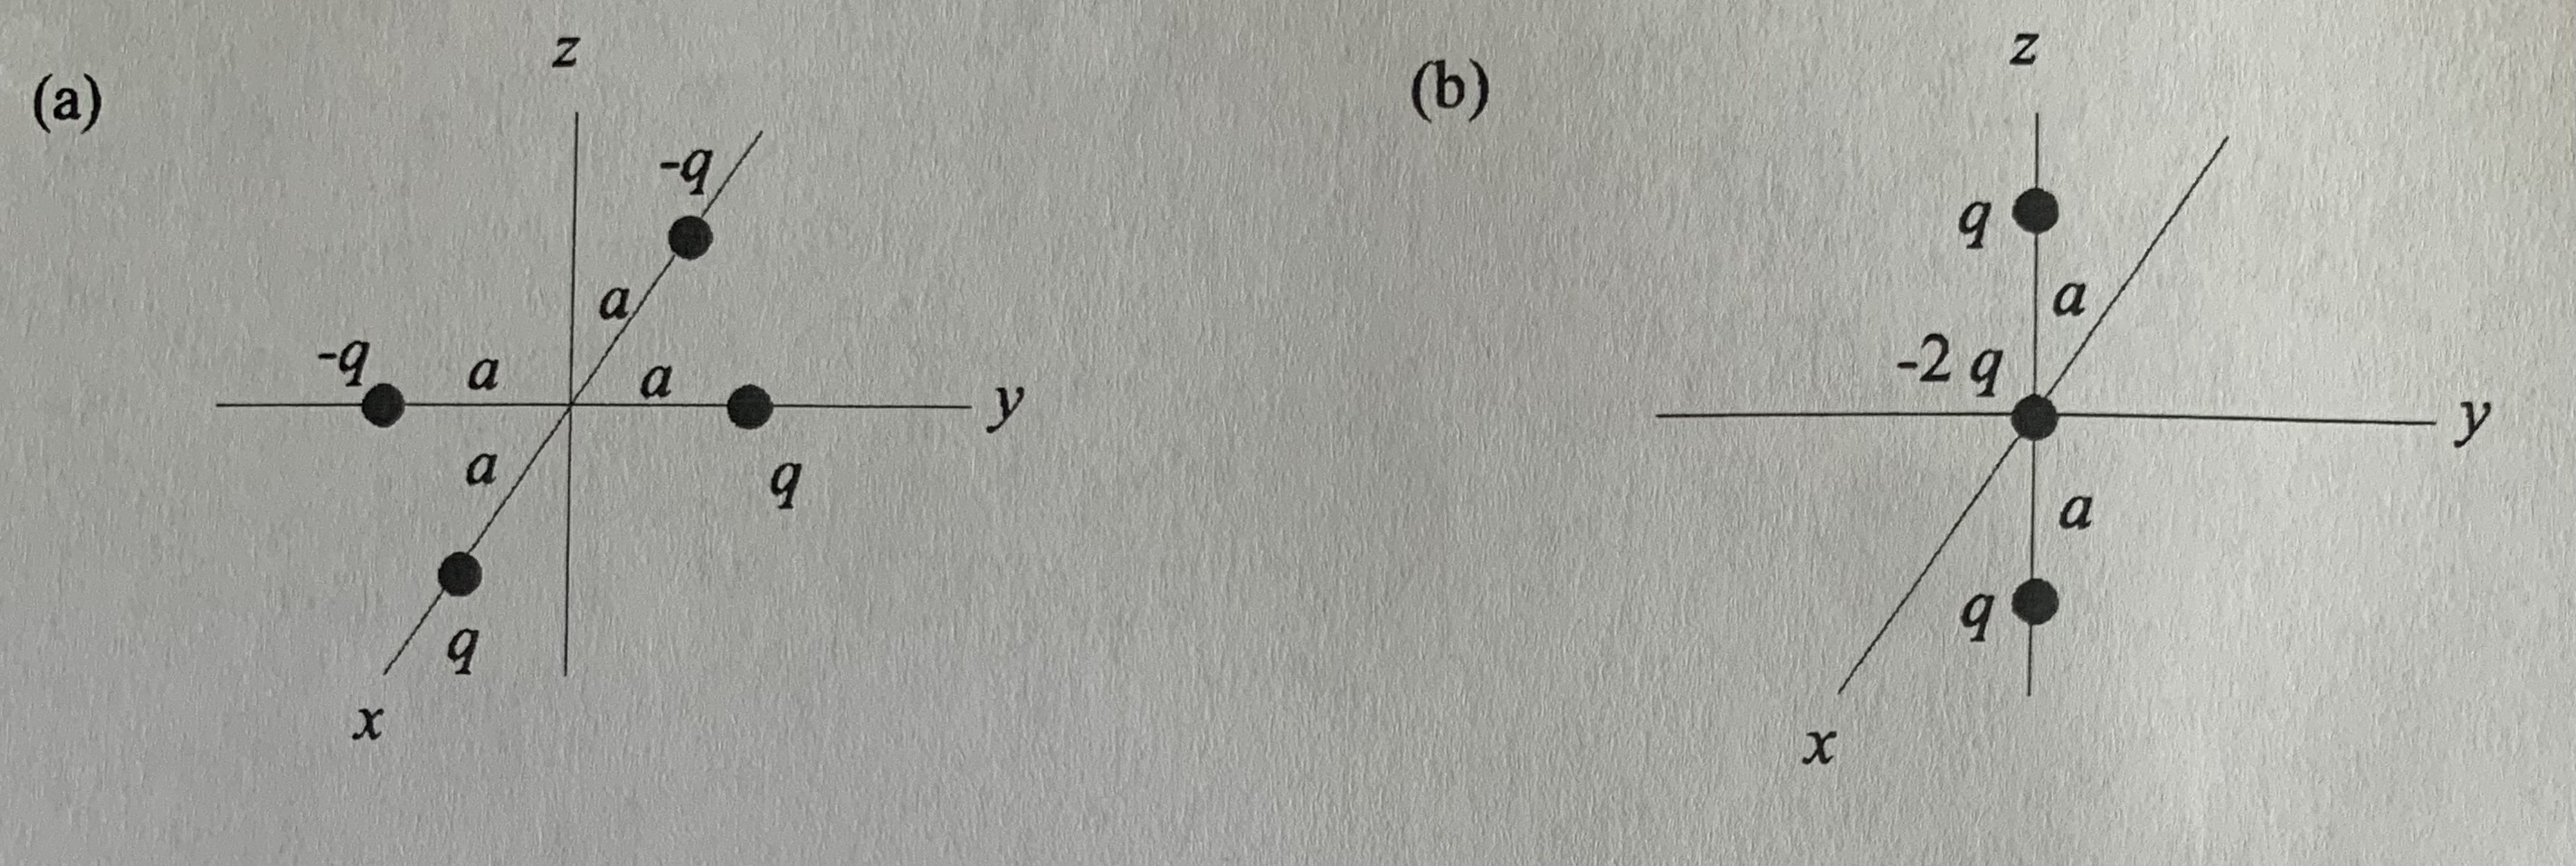
\includegraphics[width=\textwidth]{prob2.png}
   \caption{Charge configurations for parts (a) and (b).}
   \label{fig:prob2ab}
\end{figure}

\sol{

The multipole moments
\begin{eqnarray}
    q_{lm} = \int \dd[3]{\va*{r}} Y_{lm}^{*}(\theta,\phi) r^{l} \rho(\va*{r})
.\end{eqnarray}

(a) The charge configuration here is described by the charge density
\begin{eqnarray}
\begin{aligned}
    \rho(\va*{r}) &= q [ \delta(\va*{r} - a \vu*{e}_{x}) - \delta(\va*{r} + a \vu*{e}_{x}) + \delta(\va*{r} - a \vu*{e}_{y}) - \delta(\va*{r} + a \vu*{e}_{y}) ] \\
                  &= \frac{q}{a^2} \delta(r-a) \delta(\theta - \pi/2) [ \delta(\phi) - \delta(\phi - \pi) + \delta(\phi - \pi/2) - \delta(\phi - 3 \pi/2) ]
.\end{aligned}
\end{eqnarray}
The three-dimensional integration then reduces to function evaluations:
\begin{eqnarray}
\begin{aligned}
    q_{lm} &= qa^{l} \Big[ Y_{lm}^{*}(\pi/2,0) - Y_{lm}^{*}(\pi/2,\pi) + Y_{lm}^{*}(\pi/2,\pi/2) - Y_{lm}^{*}(\pi/2,3\pi/2) \Big] \\
           &= q a^{l} [ 1 - (-1)^{l} ] \Big[ Y_{lm}^{*}(\pi/2,0) + Y_{lm}^{*}(\pi/2,\pi/2) \Big]
,\end{aligned}
\end{eqnarray}
where we have used
\begin{eqnarray}
    Y_{lm}(\pi - \theta,\phi + \pi) = (-1)^{l} Y_{lm}(\pi)
,\end{eqnarray}
which translates directly upon complex conjugation.
Recall that spherical harmonics are explicitly given as 
\begin{eqnarray}
    Y_{lm}(\theta,\phi) = \sqrt{\frac{2l+1}{4\pi} \frac{(l-m)!}{(l+m)!}} P_{l}^{m}(\cos{\theta}) e^{im\phi}
,\end{eqnarray}
The moments then simplify as
\begin{eqnarray}
    q_{lm} = q a^{l} \sqrt{\frac{2l+1}{4 \pi} \frac{(l-m)!}{(l+m)!}} P_{l}^{m}(0) [ 1 - (-1)^{l} ]  [ 1 + (-i)^{m} ]
.\end{eqnarray}

From this we can glean that if $l$ or $m$ are even, then $q_{lm}$ is zero.
The first couple sets of nonzero moments are given as
\begin{gather}
    q_{11} = qa\sqrt{\frac{3}{2\pi}}(-1+i) \quad q_{10} = 0 \\
    q_{33} = qa^{3} \sqrt{\frac{35}{16 \pi}} \quad q_{32} = 0 \quad q_{31} = qa^3 \sqrt{\frac{21}{16 \pi}}(1-i) \quad q_{30} = 0
.\end{gather}
Note that $q_{l,-m} = (-1)^{m}q_{lm}^{*}$.

(b) The charge density for this charge configuration is
\begin{eqnarray}
\begin{aligned}
    \rho(\va*{r}) &= q[ \delta(\va*{r} - a \vu*{e}_{z}) -2\delta(\va*{r}) + \delta(\va*{r} + a \vu*{e}_{z}) ] \\
                  &= q \Big[ \frac{1}{2 \pi a^2}\delta(r-a) [ \delta(\cos{\theta} + 1) + \delta(\cos{\theta} - 1) ] - \frac{\delta(r)}{2 \pi r^2} \Big]
.\end{aligned}
\end{eqnarray}
Putting this into the moment definition
\begin{eqnarray}
\begin{aligned}
    q_{lm} &= q a^{l} \sqrt{\frac{2l+1}{4\pi}} \int \dd{(\cos{\theta})} P_{l}(\cos{\theta}) \Big[ \delta(\cos{\theta}-1) + \delta(\cos{\theta}+1) \Big] - \frac{q}{\sqrt{\pi}} \delta_{l 0} \delta_{m 0} \\
           &= \delta_{m 0} \Bigg[ q a^{l} \sqrt{\frac{2l+1}{4\pi}} [ 1 + (-1)^{n} ] - \frac{q}{\sqrt{\pi}} \delta_{l 0} \Bigg]
\end{aligned}
.\end{eqnarray}

(c) For the charge configuration of part (b), the multipole expansion of the potential is given as
\begin{eqnarray}
\begin{aligned}
    \Phi(\va*{r}) &= \frac{q}{\epsilon_0} \sum_{l=0}^{\infty} \frac{1}{2l+1} \Big[ a^{l} \sqrt{\frac{2l+1}{4\pi}} - \frac{1}{\sqrt{\pi}} \delta_{l 0} \Big] \frac{1}{r^{l+1}} \sqrt{\frac{2l+1}{4\pi}} P_{l}(\cos{\theta}) \\
                  &= \frac{q}{2 \pi \epsilon_0} \sum_{l=0}^{\infty} \frac{a^{2l}}{r^{2l+1}} P_{2l}(\cos{\theta}) - \frac{q}{2 \pi \epsilon_0 r}
.\end{aligned}
\end{eqnarray}
To lowest order, the potential far from the origin is
\begin{eqnarray}
    \Phi(\va*{r}) \approx \frac{q}{2\pi\epsilon_0 a} \Big( \frac{a}{r} \Big)^3 P_{2}(\cos{\theta})
.\end{eqnarray}
In the $xy$-plane, this becomes
\begin{eqnarray}
    \label{eq:xy-multipole-expansion}
    \Phi(\va*{r}) = -\frac{q}{4\pi\epsilon_0 a} \Big( \frac{a}{r} \Big)^3
.\end{eqnarray}

(d) The potential from Coulomb's law in the $xy$-plane due to the charge configuration in part (b) is given by
\begin{eqnarray}
    \label{eq:exact-coulomb}
    \Phi(\va*{r}) = \frac{q}{2 \pi \epsilon_0} \Big[ \frac{1}{\sqrt{r^2 + a^2}} - \frac{1}{r} \Big] = -\frac{q}{2 \pi \epsilon_0 a} \Big[ \frac{a}{r} - \frac{1}{\sqrt{(r/a)^2 + 1}} \Big]
.\end{eqnarray}

\begin{figure}[h!tb]
   \centering
   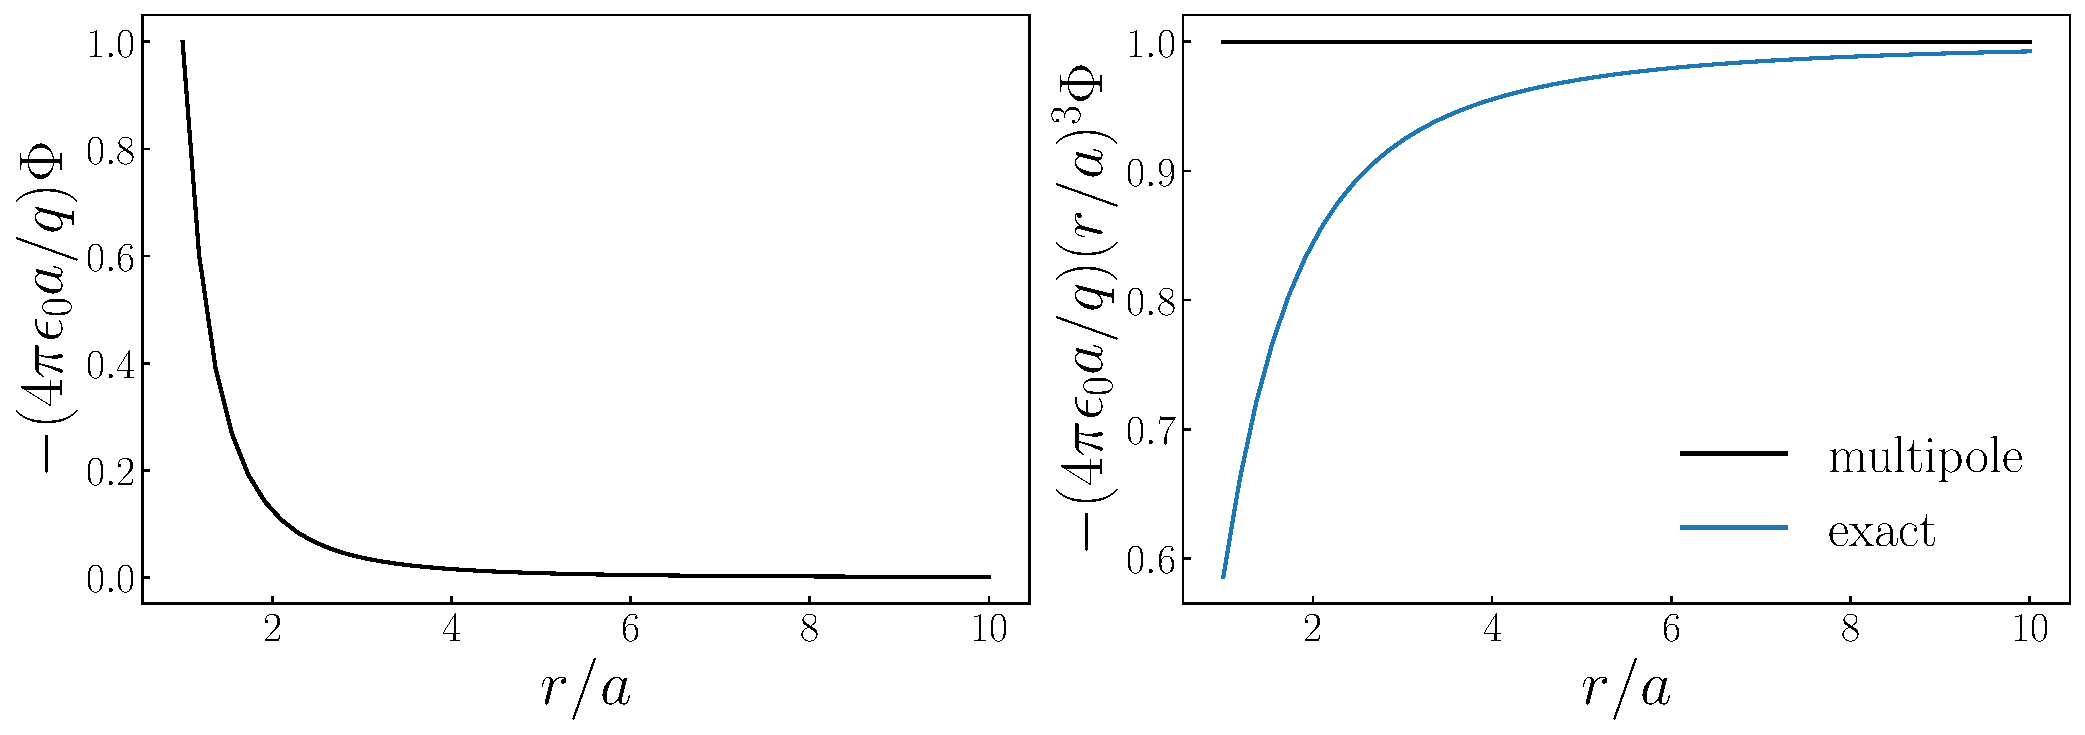
\includegraphics[width=\textwidth]{prob2.pdf}
   \caption{\textbf{[Left]} Plot of potential given in \eref{xy-multipole-expansion} and \textbf{[Right]} Plot of potential in \eref{exact-coulomb} modulated by $(a/r)^3$ asymptotic factor and \eref{xy-multipole-expansion}.}
\end{figure}



}



\end{document}
